\subsection{M.PC.10 - Indice di stabilità dei requisiti}
\begin{figure}[H]
    \centering
    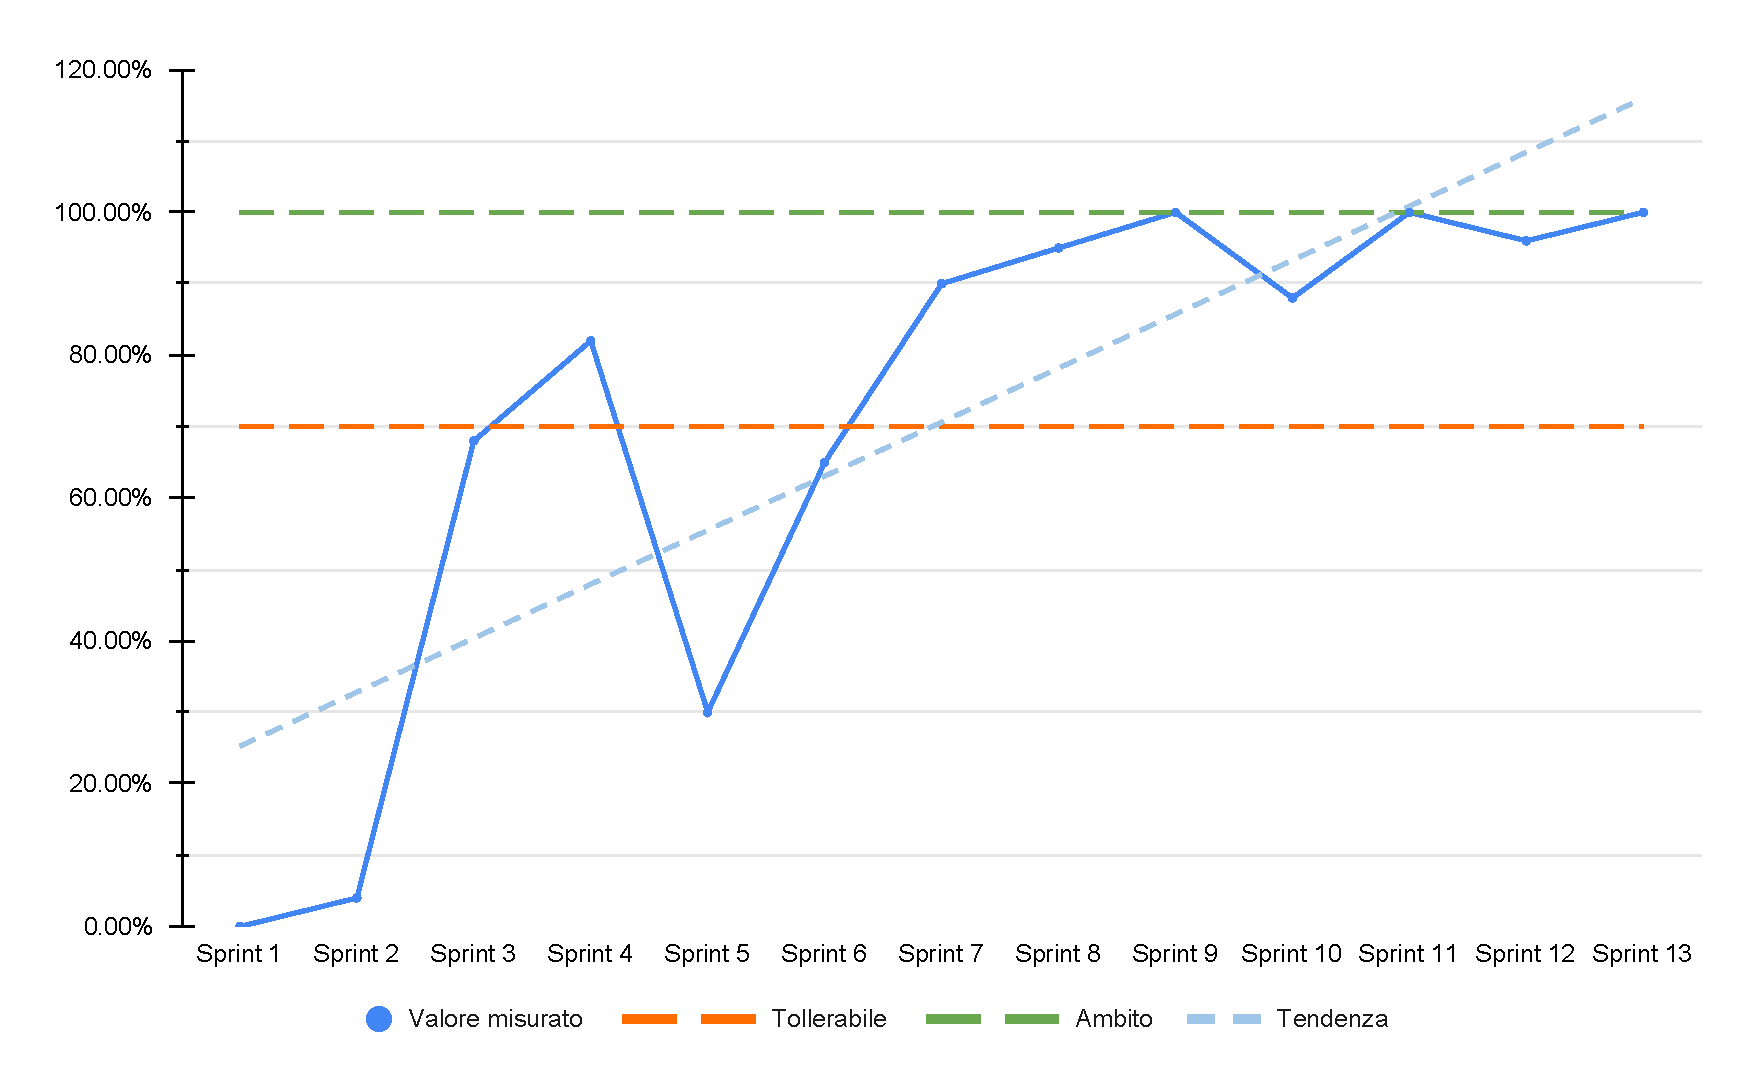
\includegraphics[width=\textwidth]{assets/stabilita_requisiti.pdf}
    \caption{M.PC.10 - Indice di stabilità dei requisiti}
\end{figure}

\par Il grafico evidenzia un'alta instabilità dei requisiti durante i primi due \glossario{sprint}, a causa dell'inesperienza del team nella definizione dei \glossario{casi d'uso} e nell'identificazione dei requisiti funzionali e non funzionali. Inoltre, sono state apportate modifiche sostanziali ai requisiti dopo l'incontro con la \glossario{Proponente}. Dal terzo \glossario{sprint}, invece, si nota un incremento nella stabilità, in quanto le modifiche hanno avuto un impatto minore. Nel quinto sprint, a seguito di un incontro con il Professor Cardin, il team ha attuato una rivisitazione completa e una ristrutturazione del documento di \AdR. Sono stati inoltre aggiunti nuovi casi d'uso e requisiti, poiché la stretta collaborazione tra i membri del team ha contribuito a chiarire le funzionalità del prodotto. Pertanto, in corrispondenza del quinto sprint, il valore misurato risulta essere nuovamente inferiore alle aspettative. A partire dal settimo sprint, il gruppo ha riportato la situazione sotto controllo, raggiungendo un livello di profondità e stabilità dei requisiti soddisfacente.

\par Durante il decimo \glossario{sprint}, il documento di \AdR\ è stato aggiornato in seguito alla revisione \glossario{RTB}. In particolare, è stato eliminato un requisito ed è stata migliorata la suddivisione tra requisiti funzionali, di vincolo e di qualità. Nel dodicesimo sprint, il team ha effettuato ulteriori aggiornamenti ai requisiti basandosi sulle osservazioni dei programmatori. Questo ha comportato la rimozione di due requisiti: la copia del messaggio di \glossario{debug} e il controllo degli errori nella descrizione del \glossario{dizionario dati}. Nonostante queste modifiche, il team è riuscito a mantenere l'indice di stabilità dei requisiti vicino al valore desiderato.
